\section{Data Flow Experiments: Supplementary Details}

This section provides additional details for the experiments presented in
Section~5.

\subsection{Models}

\paragraph{(I) Sequential Model} The inst2vec model consists of 619,650
trainable parameters in the  configuration outlined in
Figure~\ref{figure:lstm_node_level}. The model, implemented in TensorFlow, uses
the same parameters as in the original work: 2$\times$ 64 dimensional LSTM
layers followed by a 64 dimensional dense layer and the final 2 dimensional
output layer. Sequences are padded and truncated to 5k tokens and processed in
batches of 64.

\paragraph{(II) Graph Models} For CDFG and \programl approaches we use the same
model architecture. The model, implemented in PyTorch, consists of a customized
GGNN with 87,070 trainable parameters. Batches are implemented as disconnected
graphs that are constructed to enable efficient processing of graphs of
differing size in parallel without padding. We use a combined batch size of
$10,000$ vertices. If a single graph contains more than $10,000$ vertices, it is
processed on its own.

\begin{figure}
  \centering %
  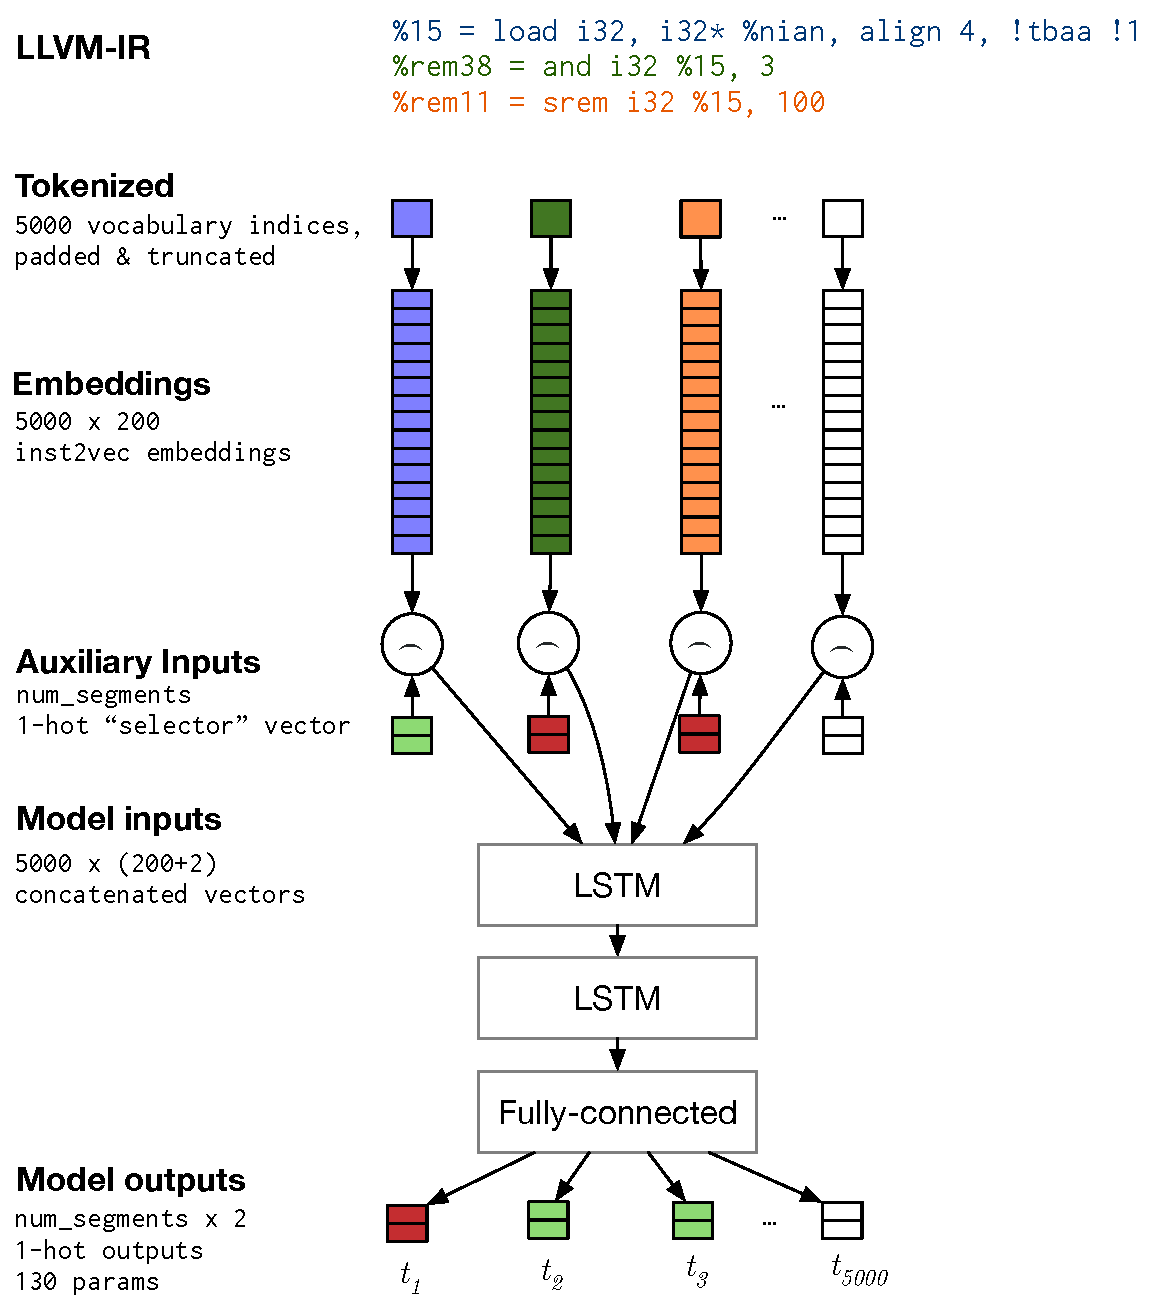
\includegraphics[width=\columnwidth]{images/lstm_node_level}%
  \caption{%
    Extending inst2vec~\citep{Ben-nun2018} to perform per-instruction
    classification of LLVM-IR. The $\frown$ operator denotes vector
    concatenation.%
  }%
  \label{figure:lstm_node_level}%
\end{figure}

\subsection{Experimental Setup}
\label{app:dataflow_experimental_setup}

\paragraph{Training Details and Parameters}
All models were trained in an end-to-end fashion with the Adam
optimizer~\citep{Kingma2015} using the default configuration and a learning rate
of $1\cdot10^{-3}$ for the LSTMs and $2.5\cdot 10^{-4}$ for the GGNNs. We
trained the models on 1M training graphs, evaluating on a fixed 10k validation
set at 10k intervals for the first 50k training graphs, and at 100k intervals
thereafter. The checkpoint with the greatest validation F$_1$ score is used for
testing.

\paragraph{Runtimes} All experiments were conducted on shared machines equipped
with an NVIDIA GTX 1080 GPU, 32GB of RAM, mechanical hard drives, and
server-grade Intel Xeon processors. Figure~\ref{tables:model_timings} provides
measurements of the average runtimes of each approach across the five DDF-30
tasks. In our implementation, we find training and testing to be I/O bound as
programs are processed faster than loading many small files from disk. In
particular, CDFG performance suffers relative to \programl as the conversion
from \programl to CDFG representations is performed on-demand. For validation,
inputs are loaded once into system memory and re-used, so the measured time
provides a more accurate estimate of processing requirements.

\begin{table*}
\centering%
\footnotesize
\begin{tabular}{r c c c c c}
  & Train time & Test time & Train time/graph & Val time/graph & Test time/graph \\
  \toprule
  inst2vec & 10h52m & 1h33m & 45ms & 3ms & 36ms\\
  CDFG & 13h14m & 3h27m & 64ms & 1ms & 62ms\\
  \programl & 7h21m & 1h39m & 26ms & 3ms & 24ms\\
\end{tabular}
\caption{Average training and inference times on DDF-30 tasks}
\label{tables:model_timings}
\end{table*}
